\documentclass[conference]{IEEEtran}
\usepackage[utf8]{vietnam}
\usepackage{amsmath,amssymb,amsfonts}
\usepackage{algorithm}
\usepackage{algorithmic}
\usepackage{graphicx}
\graphicspath{{images/}}
\usepackage{textcomp}
\usepackage{xcolor}
\usepackage{booktabs}
\usepackage{array}
\usepackage{url}
\usepackage{cite}
\usepackage{tikz}
\usetikzlibrary{arrows.meta,positioning,shapes.geometric}

\def\BibTeX{{\rm B\kern-.05em{\sc i\kern-.025em b}\kern-.08em
    T\kern-.1667em\lower.7ex\hbox{E}\kern-.125emX}}

\begin{document}

\title{
\textbf{Phát hiện bất thường log cho hạ tầng giáo dục số dựa trên Drain3 và phân tích chuỗi sự kiện}\\[0.8em]
\large\textit{Log Anomaly Detection for Digital Education Infrastructure using Drain3 and Event Sequence Analysis}
}

\author{\IEEEauthorblockN{Trịnh Hoàng Tú}
\IEEEauthorblockA{\textit{Khoa Công nghệ thông tin} \\
\textit{Trường Đại học Ngoại ngữ - Tin học TP.HCM (HUFLIT)}\\
TP. Hồ Chí Minh, Việt Nam \\
Email: tht.csec2005@gmail.com}
}

\maketitle

\begin{abstract}
Bài báo trình bày một pipeline tái lập cho phát hiện bất thường log dựa trên Drain3 và phân tích chuỗi sự kiện, đánh giá trên hai benchmark log hệ thống và định hướng chuyển giao sang hạ tầng giáo dục số. Log thô được parse thành event template, gom thành chuỗi vận hành và chấm điểm bất thường bằng bốn nhánh thay thế: PCA/TruncatedSVD reconstruction, Isolation Forest, DeepLog next-event prediction và một Transformer masked event modeling lấy cảm hứng từ LogBERT. Trên HDFS (500.000 dòng, 137 template), đánh giá 5 random seed cho thấy PCA dẫn đầu với F1 $0.5711 \pm 0.0944$, cao hơn TruncatedSVD ($0.4540 \pm 0.1366$), DeepLog top-k ($0.4608 \pm 0.0196$) và Isolation Forest ($0.1328 \pm 0.0103$). Trên BGL (500.000 dòng, 198 template, cửa sổ $W{=}100$), thứ tự đảo chiều: DeepLog đạt F1 $0.9822 \pm 0.0035$ và Transformer val-tuned đạt $0.9388 \pm 0.0080$, vượt nhẹ PCA. Hai kết quả cho thấy hiệu quả của mỗi nhánh chấm điểm phụ thuộc trực tiếp vào vocabulary, độ dài cửa sổ và tỷ lệ anomaly của dữ liệu. Đóng góp gồm: (i) pipeline đánh giá tái lập với protocol tránh rò rỉ test set; (ii) ablation study cho Drain3 threshold, DeepLog top-k và mask ratio; (iii) đánh giá chéo HDFS--BGL trên cùng pipeline; (iv) benchmark độ trễ và mapping thận trọng sang môi trường LMS đã ẩn danh.
\end{abstract}

\begin{IEEEkeywords}
Log anomaly detection, masked event modeling, Transformer, Drain3, AIOps, digital education infrastructure.
\end{IEEEkeywords}

\section{Giới thiệu}
Hạ tầng giáo dục số hiện đại tích hợp LMS, máy chủ web, cơ sở dữ liệu, hệ thống xác thực, API và dịch vụ đám mây; mỗi thành phần sinh log với định dạng và tần suất khác nhau. Log của LMS vừa phản ánh trạng thái kỹ thuật vừa thể hiện luồng nghiệp vụ đặc thù như đăng nhập hàng loạt theo lịch học, truy cập bài thi và gọi API học liệu, trong khi luật thủ công nhanh chóng lỗi thời khi hệ thống thay đổi. Bài toán phát hiện bất thường log do đó cần được xử lý ở cấp \emph{chuỗi sự kiện} thay vì từng dòng riêng lẻ.

Bài báo định vị như một nghiên cứu ứng dụng và đánh giá hệ thống, không đề xuất thuật toán anomaly detection mới. Ý tưởng trung tâm là xem \textit{chuỗi event template} như tầng biểu diễn trung gian: đủ gọn để chạy baseline nhẹ, đủ cấu trúc để mở rộng sang mô hình chuỗi, và đủ rõ ràng để ánh xạ sang các đơn vị vận hành của LMS như session, người dùng đã ẩn danh hoặc cửa sổ thời gian. Ba câu hỏi nghiên cứu được đặt ra:
\begin{itemize}
    \item \textbf{RQ1:} Cách xây dựng chuỗi event sau Drain3 ảnh hưởng như thế nào tới tín hiệu phát hiện bất thường?
    \item \textbf{RQ2:} Bốn nhánh chấm điểm (reconstruction, isolation, next-event, masked event) cho kết quả khác nhau ra sao trên cùng chuỗi event?
    \item \textbf{RQ3:} Thứ tự ưu thế của các nhánh có giữ nguyên khi chuyển từ HDFS sang BGL (đặc trưng dữ liệu rất khác) không?
\end{itemize}

Đóng góp chính gồm: (1) pipeline Drain3--event sequence--anomaly scoring với bốn nhánh chấm điểm thay thế (PCA/SVD, Isolation Forest, DeepLog, Transformer masked event modeling); (2) đánh giá đa-seed (5 random seed) trên HDFS với protocol tránh rò rỉ test set, kèm grouping strategy study cho Block ID/fixed window/sliding window; (3) đánh giá chéo HDFS--BGL trên cùng pipeline; (4) ablation cho Drain3 threshold, DeepLog top-k và Transformer mask ratio, benchmark độ trễ suy luận; (5) phân tích chi phí, lỗi dự kiến và mapping thận trọng sang LMS/cổng thông tin giáo dục đã ẩn danh.

\section{Các nghiên cứu liên quan}
\subsection{Phương pháp thống kê và học máy truyền thống}
Các phương pháp đầu tiên trong phân tích bất thường log thường biểu diễn log dưới dạng vector tần suất sự kiện hoặc ma trận đặc trưng, sau đó áp dụng PCA, clustering hoặc Isolation Forest \cite{b10,b11}. PCA được sử dụng để tách không gian hành vi bình thường và phát hiện điểm lệch khỏi không gian con chính. Nhóm phương pháp này có ưu điểm là nhẹ, dễ triển khai và không yêu cầu tài nguyên tính toán lớn. Tuy nhiên, chúng thường bỏ qua thứ tự thời gian và quan hệ ngữ cảnh giữa các sự kiện, trong khi nhiều lỗi hệ thống chỉ có ý nghĩa khi xét theo chuỗi.

\subsection{Mô hình chuỗi dựa trên RNN/LSTM}
DeepLog là một trong những công trình tiêu biểu sử dụng LSTM để học chuỗi log và dự đoán sự kiện tiếp theo \cite{b1}. Nếu sự kiện thực tế nằm ngoài nhóm dự đoán có xác suất cao, chuỗi log được xem là bất thường. LogAnomaly mở rộng hướng này bằng cách kết hợp thông tin tuần tự và định lượng của log \cite{b13}, trong khi LogRobust khai thác biểu diễn ngữ nghĩa và attention-based Bi-LSTM để xử lý log không ổn định \cite{b14}. PLELog tiếp cận bài toán theo hướng bán giám sát, dùng probabilistic label estimation để giảm phụ thuộc vào nhãn thủ công \cite{b15}. Nhìn chung, nhóm RNN/LSTM khai thác quan hệ chuỗi tốt hơn các phương pháp thống kê, nhưng vẫn chịu hạn chế của xử lý tuần tự và khó mở rộng với chuỗi dài.

\subsection{Log parsing và vai trò của Drain3}
Trước khi đưa log vào mô hình học máy, log thô cần được chuyển thành mẫu sự kiện (event template). Drain đề xuất cây phân tích cú pháp có độ sâu cố định để parse log trực tuyến với tốc độ cao \cite{b3}. Drain3 kế thừa hướng tiếp cận này và được sử dụng rộng rãi trong các pipeline AIOps nhờ khả năng xử lý log streaming. Gần đây, các phương pháp như LogPPT khai thác prompt-based few-shot learning để cải thiện log parsing khi dữ liệu gán nhãn ít hoặc template thay đổi theo miền ứng dụng \cite{b7}. Điều này cho thấy chất lượng parsing vẫn là một yếu tố quyết định trong toàn bộ hệ thống phát hiện bất thường.

\subsection{Transformer và tự giám sát trong log anomaly detection}
Transformer sử dụng Self-Attention để học quan hệ giữa mọi vị trí trong chuỗi đầu vào \cite{b4}. LogBERT áp dụng ý tưởng BERT vào log anomaly detection bằng cách học biểu diễn chuỗi log bình thường thông qua các tác vụ tự giám sát như Masked Log Message Prediction và Volume of Hypersphere Minimization \cite{b2}. Khi một chuỗi log mới lệch khỏi phân bố hành vi bình thường, mô hình có thể gán điểm bất thường cao. Các khảo sát gần đây cũng ghi nhận xu hướng chuyển từ mô hình tuần tự truyền thống sang biểu diễn học sâu và tự giám sát cho log anomaly detection \cite{b16}. Ưu điểm của LogBERT là khả năng học ngữ cảnh hai chiều và phụ thuộc dài hạn tốt hơn mô hình tuần tự truyền thống, nhưng yêu cầu pipeline tiền xử lý và gom chuỗi phải được thiết kế rõ ràng.

\subsection{Hướng prompt/LLM cho phân tích log}
Các nghiên cứu gần đây bắt đầu khai thác mô hình ngôn ngữ lớn và prompt learning cho bài toán log. LogPrompt sử dụng prompt để hỗ trợ phát hiện bất thường từ log \cite{b8}, trong khi LogGPT nghiên cứu khả năng áp dụng mô hình kiểu GPT cho log anomaly detection \cite{b9}. Các hướng này hứa hẹn cải thiện khả năng hiểu ngữ nghĩa và giải thích cảnh báo, nhưng cũng đặt ra thách thức về chi phí suy luận, độ ổn định, bảo mật dữ liệu log và khả năng triển khai trong hệ thống thời gian thực.

\begin{table}[!t]
\caption{So sánh các nhóm phương pháp phát hiện bất thường log}
\begin{center}
\scriptsize
\begin{tabular}{p{1.35cm}p{1.55cm}p{3.1cm}}
\toprule
\textbf{Nhóm} & \textbf{Đại diện} & \textbf{Nhận xét} \\
\midrule
Thống kê & PCA, Isolation Forest & Nhẹ và dễ triển khai, nhưng yếu với phụ thuộc ngữ cảnh dài. \\
Chuỗi & DeepLog, LSTM & Học thứ tự event tốt hơn, nhưng khó song song hóa và hạn chế với chuỗi dài. \\
Transformer & LogBERT & Học ngữ cảnh hai chiều, phù hợp dữ liệu log ít nhãn; cần parsing tốt và chọn ngưỡng hợp lý. \\
Prompt/LLM & LogPPT, LogPrompt, LogGPT & Có tiềm năng giải thích cảnh báo, nhưng chi phí cao và cần kiểm soát dữ liệu nhạy cảm. \\
\bottomrule
\end{tabular}
\label{tab_related_work}
\end{center}
\end{table}

\subsection{Khoảng trống nghiên cứu}
Từ các công trình liên quan, có thể rút ra bốn khoảng trống chính. Thứ nhất, các phương pháp thống kê và học máy truyền thống như PCA hoặc Isolation Forest nhẹ và dễ triển khai, nhưng thường xem log như vector tần suất nên khó nắm bắt thứ tự sự kiện. Thứ hai, các mô hình chuỗi như DeepLog, LogAnomaly, LogRobust và PLELog đã cải thiện khả năng học quan hệ tuần tự hoặc ngữ nghĩa, nhưng vẫn phụ thuộc vào kiến trúc tuần tự, chất lượng nhãn hoặc tính ổn định của log \cite{b1,b13,b14,b15}. Thứ ba, các mô hình Transformer như LogBERT có khả năng học ngữ cảnh hai chiều, nhưng hiệu quả phụ thuộc mạnh vào chất lượng bước log parsing và cách gom chuỗi \cite{b2}. Thứ tư, phần lớn benchmark log anomaly detection tập trung vào hệ thống hạ tầng như HDFS/BGL; việc ánh xạ pipeline này sang LMS cần làm rõ đơn vị gom chuỗi, ràng buộc riêng tư dữ liệu và các kịch bản nghiệp vụ giáo dục số.

\begin{table}[!t]
\caption{Research gaps rút ra từ các hướng nghiên cứu liên quan}
\begin{center}
\scriptsize
\begin{tabular}{>{\raggedright\arraybackslash}p{1.5cm}>{\raggedright\arraybackslash}p{1.5cm}>{\raggedright\arraybackslash}p{1.8cm}>{\raggedright\arraybackslash}p{1.8cm}}
\toprule
\textbf{Hướng} & \textbf{Điểm mạnh} & \textbf{Khoảng trống} & \textbf{Cải thiện trong bài} \\
\midrule
PCA/IF & Nhẹ, dễ tái lập & Không học thứ tự event & Đo baseline để lượng hóa giới hạn \\
DeepLog, LogAnomaly & Học quan hệ chuỗi & Hạn chế với chuỗi dài, log biến động & Làm nền so sánh cho mô hình ngữ cảnh \\
LogRobust, PLELog & Xử lý semantic hoặc nhãn yếu & Vẫn cần pipeline parsing và gom chuỗi rõ & Tách rõ parsing, grouping, scoring \\
LogBERT & Học ngữ cảnh hai chiều & Phụ thuộc chất lượng event sequence & Chọn Drain3 trước LogBERT \\
LMS & Bối cảnh ứng dụng thực tế & Thiếu log công khai, dữ liệu nhạy cảm & Giới hạn scope và đề xuất mapping ẩn danh \\
\bottomrule
\end{tabular}
\label{tab_research_gaps}
\end{center}
\end{table}

Do đó, bài báo không chỉ chọn một mô hình học sâu đơn lẻ mà xây dựng pipeline gồm hai thành phần chính. Drain3 được chọn vì log LMS và log hạ tầng đều chứa nhiều tham số runtime biến đổi; nếu không parse trước, không gian token sẽ lớn và nhiễu. Một Transformer masked event modeling lấy cảm hứng từ LogBERT \cite{b2} được xem là hướng mở rộng hứa hẹn vì có khả năng mô hình hóa phụ thuộc ngữ cảnh dài hạn trong chuỗi event, nơi quan hệ giữa các sự kiện quan trọng hơn từng dòng log riêng lẻ. Các baseline PCA, TruncatedSVD và Isolation Forest được dùng để định lượng mức hiệu quả của các phương pháp nhẹ trước khi mở rộng sang mô hình Transformer. Kết quả đo lường được báo cáo bằng Precision, Recall và F1-score với trung bình $\pm$ độ lệch chuẩn trên 5 random seed, nhờ đó đóng góp của pipeline có thể được đánh giá và kiểm chứng thay vì chỉ mô tả định tính.

\section{Phương pháp đề xuất}
\subsection{Tổng quan pipeline}
Pipeline đề xuất được thiết kế theo hướng tách rõ ba tầng xử lý: chuẩn hóa log, xây dựng chuỗi sự kiện và phát hiện bất thường. Đầu vào là tập log thô $L=\{l_1,l_2,\ldots,l_N\}$ sinh ra từ hệ thống vận hành. Đầu ra là nhãn hoặc điểm bất thường $a(S)$ cho từng chuỗi sự kiện $S$. Trong thực nghiệm HDFS, một chuỗi tương ứng với một Block ID; trong môi trường giáo dục số, chuỗi có thể tương ứng với một phiên đăng nhập, một người dùng đã ẩn danh, một dịch vụ hoặc một cửa sổ thời gian.

\begin{figure}[!t]
\centering
\resizebox{\columnwidth}{!}{
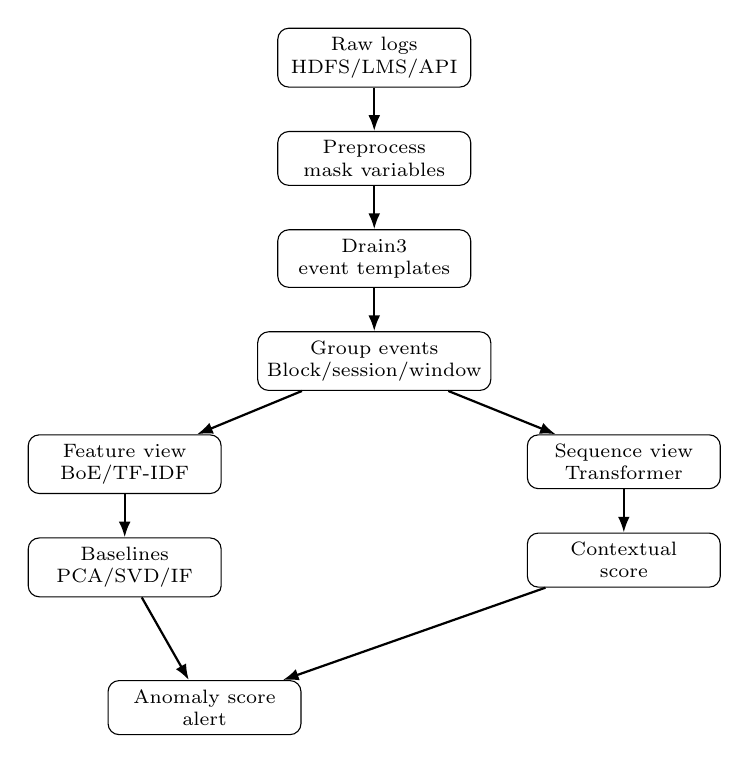
\begin{tikzpicture}[
    node distance=0.55cm and 0.45cm,
    box/.style={rectangle, draw, rounded corners, align=center, minimum width=2.45cm, minimum height=0.62cm, font=\scriptsize},
    arrow/.style={-{Latex[length=2mm]}, thick}
]
\node[box] (raw) {Raw logs\\HDFS/LMS/API};
\node[box, below=of raw] (pre) {Preprocess\\mask variables};
\node[box, below=of pre] (parse) {Drain3\\event templates};
\node[box, below=of parse] (seq) {Group events\\Block/session/window};
\node[box, below left=of seq] (vec) {Feature view\\BoE/TF-IDF};
\node[box, below=of vec] (base) {Baselines\\PCA/SVD/IF};
\node[box, below right=of seq] (bert) {Sequence view\\Transformer};
\node[box, below=of bert] (seqscore) {Contextual\\score};
\node[box, below right=1.05cm and -1.45cm of base] (score) {Anomaly score\\alert};
\draw[arrow] (raw) -- (pre);
\draw[arrow] (pre) -- (parse);
\draw[arrow] (parse) -- (seq);
\draw[arrow] (seq) -- (vec);
\draw[arrow] (vec) -- (base);
\draw[arrow] (seq) -- (bert);
\draw[arrow] (bert) -- (seqscore);
\draw[arrow] (base) -- (score);
\draw[arrow] (seqscore) -- (score);
\end{tikzpicture}
}
\caption{Sơ đồ pipeline phát hiện bất thường log đề xuất}
\label{fig_pipeline}
\end{figure}

Quy trình tổng thể gồm sáu bước:
\begin{itemize}
    \item \textbf{Bước 1 -- Thu thập log:} nhận log từ hệ thống nguồn như HDFS, LMS, API gateway hoặc máy chủ xác thực.
    \item \textbf{Bước 2 -- Tiền xử lý:} chuẩn hóa các trường biến đổi như timestamp, IP, user ID, session ID và tham số truy vấn.
    \item \textbf{Bước 3 -- Parse log:} dùng Drain3 để ánh xạ mỗi dòng log thành một event template và event ID.
    \item \textbf{Bước 4 -- Gom chuỗi:} gom các event ID theo Block ID hoặc theo session/time window để tạo chuỗi sự kiện.
    \item \textbf{Bước 5 -- Biểu diễn đặc trưng:} tạo biểu diễn bag-of-events/TF-IDF cho baseline hoặc giữ nguyên chuỗi event cho Transformer masked event modeling.
    \item \textbf{Bước 6 -- Phát hiện bất thường:} tính điểm bất thường bằng reconstruction error, Isolation Forest hoặc mô hình học chuỗi.
\end{itemize}

\begin{table}[!t]
\caption{Các bước chính của pipeline đề xuất}
\begin{center}
\scriptsize
\begin{tabular}{p{1.35cm}p{2.0cm}p{2.5cm}}
\toprule
\textbf{Bước} & \textbf{Đầu vào} & \textbf{Đầu ra} \\
\midrule
Tiền xử lý & Log thô & Log đã chuẩn hóa tham số biến đổi \\
Drain3 & Log đã chuẩn hóa & Event template và event ID \\
Gom chuỗi & Event ID & Chuỗi theo Block ID/session/window \\
Vector hóa & Chuỗi event & Bag-of-events hoặc TF-IDF vector \\
Baseline & Vector đặc trưng & Reconstruction/anomaly score \\
Transformer (LogBERT-inspired) & Chuỗi event & Contextual anomaly score \\
\bottomrule
\end{tabular}
\label{tab_pipeline}
\end{center}
\end{table}

Trong định hướng hạ tầng giáo dục số, pipeline này có thể được chuyển sang các nguồn như LMS, API gateway, reverse proxy, hệ thống xác thực, cơ sở dữ liệu và máy chủ ứng dụng sau khi log được ẩn danh. Thay vì xây dựng luật riêng cho từng nguồn log, hệ thống học pattern vận hành bình thường từ chuỗi sự kiện và đánh dấu các chuỗi lệch khỏi pattern đó. Khả năng chuyển giao này cần được xác nhận bằng log LMS thật trong giai đoạn tiếp theo.

\subsection{Phân tích cú pháp với Drain3}
Drain3 được sử dụng để tách log phi cấu trúc thành các mẫu (templates). Một dòng log thường bao gồm phần cố định mô tả loại sự kiện và phần biến đổi phát sinh khi chạy hệ thống. Drain3 giữ lại phần cố định và thay các giá trị biến đổi bằng ký hiệu wildcard. Ví dụ:
\begin{itemize}
    \item Log thô: \texttt{User student\_01 login failed from 192.168.1.10}
    \item Template: \texttt{User <*> login failed from <*>}
\end{itemize}

Độ tương đồng giữa hai dòng log $T_1, T_2$ được tính theo công thức:
\begin{equation}
Sim(T_1, T_2) = \frac{\sum_{i=1}^{n} equ(t_{1,i}, t_{2,i})}{n}
\label{eq_sim}
\end{equation}
Trong đó $n$ là số lượng token và $equ$ trả về 1 nếu hai token tương ứng giống nhau, ngược lại trả về 0. Nếu độ tương đồng giữa dòng log mới và template hiện có lớn hơn ngưỡng $st$, dòng log được gán vào template đó; nếu không, Drain3 tạo template mới. Trong thực nghiệm, chúng tôi đặt $st=0.5$ và độ sâu cây bằng 4. Cấu hình này tạo 137 event template từ 500.000 dòng HDFS, cho thấy không gian event sau parsing đủ gọn để huấn luyện mô hình phía sau. Các tham số này cần được tinh chỉnh lại khi chuyển sang log thực tế của LMS vì format log có thể khác đáng kể giữa Moodle, Canvas, hệ thống tự phát triển và dịch vụ đám mây.

\subsection{Biểu diễn chuỗi log}
Sau khi parsing, mỗi template được ánh xạ thành một event ID. Một đơn vị vận hành được biểu diễn thành chuỗi:
\begin{equation}
S = [E_1, E_2, ..., E_m]
\end{equation}
Với dữ liệu HDFS, chúng tôi gom các event theo Block ID vì nhãn bất thường của benchmark được xác định ở cấp block. Một block có thể có chuỗi ví dụ như \texttt{E12 E7 E7 E19 E3}. Với dữ liệu LMS, chuỗi có thể được gom theo session ID, user ID đã ẩn danh, địa chỉ dịch vụ hoặc cửa sổ thời gian cố định. Việc chọn chiến lược gom chuỗi ảnh hưởng trực tiếp tới khả năng phát hiện bất thường: cửa sổ quá ngắn có thể bỏ lỡ tấn công kéo dài, trong khi cửa sổ quá dài có thể làm nhiễu ngữ cảnh.

Để biến lựa chọn này thành một câu hỏi thực nghiệm, notebook bổ sung một grouping strategy study. Ngoài Block ID, bài kiểm tra các chiến lược fixed window và sliding window trên cùng event stream. Với fixed window, mỗi $w$ dòng log liên tiếp tạo thành một chuỗi; với sliding window, cửa sổ kích thước $w$ trượt theo stride $s$. Nhãn của một cửa sổ được gán là bất thường nếu trong cửa sổ có ít nhất một dòng log bất thường. Tất cả chiến lược grouping được đánh giá bằng cùng một PCA reconstruction baseline để cô lập ảnh hưởng của cách xây dựng chuỗi, thay vì trộn lẫn với khác biệt kiến trúc mô hình.

\subsection{Vector hóa và baseline phát hiện bất thường}
Để đánh giá pipeline trước khi huấn luyện mô hình Transformer, chúng tôi xây dựng các baseline nhẹ trên biểu diễn vector của chuỗi event. Với PCA và TruncatedSVD, mỗi chuỗi được chuyển thành vector bag-of-events:
\begin{equation}
x_j = count(E_j, S)
\end{equation}
Trong đó $x_j$ là số lần event $E_j$ xuất hiện trong chuỗi $S$. PCA và TruncatedSVD được huấn luyện trên các chuỗi bình thường để học không gian hành vi chuẩn. Điểm bất thường được tính bằng reconstruction error:
\begin{equation}
score(S)=\frac{1}{d}\sum_{j=1}^{d}(x_j-\hat{x}_j)^2
\label{eq_reconstruction}
\end{equation}
Trong đó $x$ là vector gốc, $\hat{x}$ là vector được tái tạo sau khi chiếu qua không gian chiều thấp, và $d$ là số chiều đặc trưng. Ngưỡng bất thường được chọn bằng percentile 95 của reconstruction error trên tập huấn luyện bình thường để tránh rò rỉ thông tin từ tập kiểm thử.

Với Isolation Forest, chuỗi event được vector hóa bằng TF-IDF để giảm ảnh hưởng của các event xuất hiện quá phổ biến. Mô hình cố gắng cô lập các điểm dữ liệu khác biệt bằng các phép chia ngẫu nhiên. Do Isolation Forest không mô hình hóa thứ tự event, kết quả của nó đóng vai trò baseline cho nhóm phương pháp không học phụ thuộc chuỗi.

\subsection{Baseline chuỗi DeepLog}
\label{sec:deeplog}
Để đặt Transformer masked event modeling trong tương quan với một mô hình chuỗi truyền thống, chúng tôi tái lập DeepLog \cite{b1} dưới dạng next-event prediction bằng LSTM. Với mỗi vị trí $i$ trong chuỗi event, mô hình dự đoán $E_i$ từ cửa sổ trượt $g$ event trước đó:
\begin{equation}
\hat{P}(E_i \mid E_{i-g}, \ldots, E_{i-1}) = \text{softmax}(W_o h_i + b_o),
\end{equation}
trong đó $h_i$ là biểu diễn ẩn cuối cùng của LSTM hai lớp, hidden size 64, embedding 64, dropout 0.1. Mô hình được huấn luyện chỉ trên chuỗi bình thường bằng cross-entropy với Adam, learning rate $1\times 10^{-3}$, batch size 256 và 10 epoch. Hai chế độ chấm điểm được báo cáo. Với chế độ \textit{top-k} gốc của DeepLog, một vị trí được xem là bất thường nếu $E_i$ không thuộc tốp $K{=}9$ dự đoán; chuỗi bị gắn cảnh báo nếu có ít nhất một vị trí bất thường. Với chế độ \textit{NLL threshold}, $score(S)$ là trung bình $-\log \hat{P}(E_i)$ trên các vị trí của chuỗi, ngưỡng được chọn bằng percentile 95 trên các chuỗi validation bình thường, đồng nhất với các baseline khác.

\subsection{Hàm quyết định bất thường}
\label{sec:decision}
Mọi nhánh trong pipeline đều quy về một hàm chấm điểm $score: \mathcal{S} \rightarrow \mathbb{R}$ và một ngưỡng $\tau$. Cụ thể, với PCA và TruncatedSVD, $score(S)$ là reconstruction error trong \eqref{eq_reconstruction}; với Isolation Forest, $score(S)=-\text{decision\_function}(S)$ sao cho điểm cao tương ứng với khả năng bất thường lớn hơn; với Transformer masked event modeling, $score(S)$ là trung bình masked reconstruction loss trong \eqref{eq_loss} trên tập vị trí bị mask. Ngưỡng $\tau$ luôn được chọn từ phân phối điểm của chuỗi bình thường trong tập huấn luyện hoặc tập validation, không từ tập kiểm thử. Quyết định cuối cùng được định nghĩa thống nhất là
\begin{equation}
\hat{y}(S)=
\begin{cases}
1, & \text{nếu } score(S) > \tau,\\
0, & \text{ngược lại},
\end{cases}
\label{eq_decision}
\end{equation}
trong đó $\hat{y}(S)=1$ tương ứng với chuỗi bị gắn cảnh báo bất thường. Cách trình bày này giúp tách bạch ba thành phần: hàm chấm điểm (phụ thuộc mô hình), chiến lược chọn ngưỡng (phụ thuộc dữ liệu) và quy tắc quyết định (chung cho mọi mô hình).

\subsection{Kiến trúc Transformer masked event modeling (LogBERT-inspired)}
Phần này mô tả nhánh học chuỗi của pipeline. Chúng tôi sử dụng một Transformer Encoder kết hợp masked event modeling, lấy cảm hứng từ LogBERT \cite{b2} nhưng không tái lập đầy đủ mã nguồn và objective gốc (ví dụ hypersphere objective). Transformer Encoder được dùng để học biểu diễn hai chiều cho chuỗi event. Cơ chế Self-Attention được tính như sau:
\begin{equation}
Attention(Q,K,V) = \text{softmax}\left(\frac{QK^T}{\sqrt{d_k}}\right)V
\label{eq_att}
\end{equation}
Trong đó $Q$, $K$, $V$ lần lượt là ma trận truy vấn, khóa và giá trị. Cơ chế này cho phép mỗi event trong chuỗi tham chiếu tới toàn bộ event khác, nhờ đó mô hình có thể phát hiện những bất thường không biểu hiện bằng một dòng log đơn lẻ mà nằm ở quan hệ giữa nhiều sự kiện.

Quá trình huấn luyện sử dụng cơ chế Masked Log Key Prediction. Một tỷ lệ event trong chuỗi được thay bằng token \texttt{[MASK]}, sau đó mô hình học cách khôi phục event bị che dựa trên ngữ cảnh:
\begin{equation}
L_{MLM} = -\sum_{i \in M} \log P(k_i | S_{masked})
\label{eq_loss}
\end{equation}
Trong đó $M$ là tập vị trí bị mask, $k_i$ là event thực tại vị trí $i$. Khi inference, chuỗi có xác suất khôi phục thấp hoặc chứa event mới hiếm gặp sẽ được gán điểm bất thường cao. So với bag-of-events, Transformer masked event modeling giữ lại thứ tự event và học quan hệ ngữ cảnh hai chiều, do đó phù hợp hơn với các bất thường xuất hiện theo chuỗi hành vi. Hàm quyết định cuối cùng cho chuỗi $S$ áp dụng chung cho mọi nhánh phát hiện bất thường được định nghĩa ở mục~\ref{sec:decision}.

\begin{figure}[!t]
\centering
\resizebox{\columnwidth}{!}{
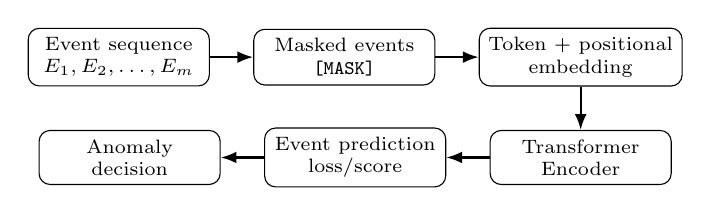
\begin{tikzpicture}[
    node distance=0.55cm,
    box/.style={rectangle, draw, rounded corners, align=center, minimum width=2.3cm, minimum height=0.62cm, font=\scriptsize},
    arrow/.style={-{Latex[length=2mm]}, thick}
]
\node[box] (seq) {Event sequence\\$E_1,E_2,\ldots,E_m$};
\node[box, right=of seq] (mask) {Masked events\\\texttt{[MASK]}};
\node[box, right=of mask] (emb) {Token + positional\\embedding};
\node[box, below=of emb] (enc) {Transformer\\Encoder};
\node[box, left=of enc] (pred) {Event prediction\\loss/score};
\node[box, left=of pred] (alert) {Anomaly\\decision};
\draw[arrow] (seq) -- (mask);
\draw[arrow] (mask) -- (emb);
\draw[arrow] (emb) -- (enc);
\draw[arrow] (enc) -- (pred);
\draw[arrow] (pred) -- (alert);
\end{tikzpicture}
}
\caption{Kiến trúc thử nghiệm Transformer masked event modeling}
\label{fig_transformer_arch}
\end{figure}

\subsection{Thuật toán tổng quát}
\begin{algorithm}[!t]
\caption{Pipeline phát hiện bất thường log}
\begin{algorithmic}[1]
\STATE Input: Tập log thô $L$, khóa gom chuỗi $g$ (Block ID/session/window)
\STATE Chuẩn hóa tham số biến đổi trong từng dòng log
\STATE Parse từng dòng log bằng Drain3 để thu event ID
\STATE Gom event ID theo khóa $g$ để tạo tập chuỗi $\mathcal{S}$
\FOR{mỗi chuỗi $S \in \mathcal{S}$}
    \STATE Tạo vector bag-of-events/TF-IDF cho baseline
    \STATE Tính reconstruction score hoặc Isolation Forest score
    \STATE Với Transformer masked event modeling, đưa chuỗi event vào Transformer Encoder
    \STATE Gán nhãn anomaly nếu $score(S) > \tau$
\ENDFOR
\STATE Output: Điểm bất thường và nhãn dự đoán cho từng chuỗi
\end{algorithmic}
\end{algorithm}

\section{Thiết lập thực nghiệm}
\subsection{Bộ dữ liệu}
Nghiên cứu sử dụng bộ dữ liệu chuẩn HDFS từ LogHub để đánh giá khả năng phát hiện bất thường trong môi trường hệ thống lớn \cite{b6,b12}. HDFS chứa log từ hệ thống Hadoop Distributed File System và được gán nhãn theo Block ID. Một block được xem là bất thường nếu chuỗi log liên quan tới block đó chứa sự kiện lỗi. Trong thực nghiệm tái lập, chúng tôi sử dụng 500.000 dòng đầu từ bản đóng gói HDFS\_v1 có nhãn trên HuggingFace nhằm kiểm tra pipeline tiền xử lý và các baseline trong điều kiện tài nguyên hạn chế.

\begin{table}[!t]
\caption{Thống kê dữ liệu HDFS sử dụng trong thực nghiệm}
\begin{center}
\begin{tabular}{lc}
\toprule
\textbf{Thông tin} & \textbf{Giá trị} \\
\midrule
Số dòng log đã parse & 500.000 \\
Số block sau khi gom chuỗi & 36.305 \\
Số block bình thường & 34.558 \\
Số block bất thường & 1.747 \\
Số event template sinh bởi Drain3 & 137 \\
Độ dài chuỗi trung bình & 13.77 event \\
Độ lệch chuẩn độ dài chuỗi & 3.45 \\
Độ dài chuỗi nhỏ nhất/lớn nhất & 2 / 269 \\
Similarity threshold & 0.5 \\
Drain depth & 4 \\
\bottomrule
\end{tabular}
\label{tab_dataset_stats}
\end{center}
\end{table}

Để kiểm tra mức độ khái quát của pipeline, chúng tôi đánh giá lại trên bộ log siêu máy tính BGL \cite{b18,b12}, sử dụng 500.000 dòng đầu từ bản đóng gói BGL trên HuggingFace. Khác với HDFS, BGL không có Block ID nên chuỗi event được gom theo cửa sổ không chồng lấn $W{=}100$ dòng, mỗi cửa sổ được gắn nhãn anomaly nếu chứa ít nhất một dòng có nhãn alert. Bảng \ref{tab_bgl_stats} tóm tắt thống kê BGL sau bước Drain3. Hai bộ dữ liệu này không phải log giáo dục, nhưng phù hợp để đánh giá năng lực học pattern vận hành của pipeline trên log hệ thống quy mô lớn.

\begin{table}[!t]
\caption{Thống kê dữ liệu BGL sử dụng trong đánh giá chéo}
\begin{center}
\begin{tabular}{lc}
\toprule
\textbf{Thông tin} & \textbf{Giá trị} \\
\midrule
Số dòng log đã parse & 500.000 \\
Cửa sổ sau khi gom & 5.000 \\
Cửa sổ bình thường & 2.657 \\
Cửa sổ bất thường & 2.343 \\
Số event template sinh bởi Drain3 & 198 \\
Kích thước cửa sổ $W$ & 100 dòng \\
Similarity threshold & 0.5 \\
Drain depth & 4 \\
\bottomrule
\end{tabular}
\label{tab_bgl_stats}
\end{center}
\end{table}

Đối với định hướng giáo dục số, dữ liệu LMS thực tế nên được thu thập trong giai đoạn tiếp theo từ máy chủ web, API gateway, database, hệ thống xác thực và dịch vụ cloud. Do log giáo dục có thể chứa thông tin cá nhân, các trường như user ID, email, IP và session ID cần được ẩn danh trước khi huấn luyện.

\subsection{Môi trường thực thi}
Cấu hình tham chiếu cho thực nghiệm:
\begin{itemize}
    \item \textbf{Phần cứng:} CPU Intel Core i7-13620H, GPU NVIDIA RTX 4050 6GB, RAM 16GB.
    \item \textbf{Phần mềm:} Ubuntu 22.04, Python 3.9, PyTorch 2.0.
\end{itemize}

\subsection{Tái lập và artifact thực nghiệm}
Để hỗ trợ kiểm chứng, thực nghiệm được tổ chức thành hai notebook độc lập. Notebook thứ nhất tái lập pipeline Drain3, vector hóa chuỗi event và các baseline PCA, TruncatedSVD, Isolation Forest; notebook này cũng bổ sung grouping strategy study để so sánh Block ID, fixed window và sliding window. Notebook thứ hai triển khai thử nghiệm Transformer masked event modeling dựa trên PyTorch để đánh giá hướng mở rộng theo LogBERT-style. Cả hai notebook đều cố định random seed bằng 42, ghi lại tham số Drain3, số dòng log, số block, số event template, metric Precision/Recall/F1 và xuất các artifact như bảng kết quả, template summary, ROC/PR curve, phân tích độ nhạy ngưỡng và kết quả grouping. Nhờ đó, các kết quả trong bài có thể được chạy lại và đối chiếu thay vì chỉ mô tả định tính.

\subsection{Quy trình tái lập thực nghiệm}
Để bảo đảm khả năng tái lập, quy trình thực nghiệm được thiết kế theo các bước cố định và triển khai bằng Python trên Google Colab. Với HDFS, log được gom theo Block ID; một block được gán nhãn bất thường nếu có ít nhất một dòng log thuộc block đó được đánh dấu lỗi. Mỗi block được biểu diễn thành chuỗi định danh sự kiện dạng \texttt{E12 E7 E7 E19 E3}; các baseline PCA và TruncatedSVD sử dụng biểu diễn bag-of-events từ chuỗi này, trong khi Isolation Forest sử dụng đặc trưng TF-IDF. Tập huấn luyện ưu tiên sử dụng log bình thường để phù hợp với giả định thực tế: hệ thống thường có nhiều dữ liệu vận hành bình thường hơn dữ liệu tấn công đã gán nhãn.

Các bước thực nghiệm gồm:
\begin{itemize}
    \item Parse log thô bằng Drain3 để sinh event template và event ID.
    \item Gom event ID thành chuỗi theo Block ID hoặc cửa sổ thời gian.
    \item Huấn luyện hoặc đánh giá mô hình phát hiện bất thường trên chuỗi event.
    \item Tính điểm bất thường cho chuỗi kiểm thử và chọn ngưỡng cảnh báo.
    \item So sánh các baseline gồm PCA reconstruction error, TruncatedSVD reconstruction error và Isolation Forest trên đặc trưng TF-IDF; Transformer masked event modeling (LogBERT-inspired) được phân tích như hướng mở rộng cho mô hình chuỗi.
\end{itemize}

Trong trường hợp chưa có log LMS thực tế, kết quả trên HDFS đóng vai trò kiểm chứng bước đầu ở cấp hạ tầng hệ thống. Khi có dữ liệu giáo dục đã ẩn danh, cùng một quy trình có thể được áp dụng lại với chiến lược gom chuỗi theo session ID, user ID ẩn danh hoặc cửa sổ thời gian.

\subsection{Chi tiết protocol và tham số}
Để tránh mơ hồ trong bước đánh giá, các thiết lập chính được cố định như sau. Với notebook baseline, dữ liệu HDFS sau khi gom theo Block ID được chia train/test theo tỷ lệ 70/30, dùng stratified split và random seed 42. PCA và TruncatedSVD được huấn luyện trên các block bình thường của tập train; ngưỡng bất thường được chọn bằng percentile 95 của reconstruction error trên chính tập train bình thường, không dùng phân phối điểm của tập test. PCA sử dụng 20 thành phần chính trên biểu diễn bag-of-events dạng dense sau chuẩn hóa; TruncatedSVD sử dụng 20 thành phần trên ma trận sparse bag-of-events. Isolation Forest dùng TF-IDF mặc định của \texttt{scikit-learn}, số cây 200, random seed 42, và tham số contamination được đặt theo tỷ lệ anomaly trong tập train, giới hạn trong khoảng $[0.001, 0.2]$.

Với thử nghiệm Transformer, dữ liệu 200.000 dòng HDFS được chia train/validation/test theo tỷ lệ 60/20/20. Mô hình chỉ huấn luyện trên chuỗi bình thường của tập train bằng masked event modeling với mask ratio 0.15. Ngưỡng không giám sát được chọn bằng percentile 95 của masked reconstruction loss trên các chuỗi validation bình thường. Cấu hình chọn ngưỡng bằng validation labels được báo cáo riêng như tham khảo, không được xem là thiết lập hoàn toàn không giám sát.

\subsection{Độ đo đánh giá}
Do dữ liệu log thường mất cân bằng, accuracy không đủ phản ánh chất lượng mô hình. Bài báo sử dụng Precision, Recall và F1-score:
\begin{equation}
Precision = \frac{TP}{TP + FP}
\end{equation}
\begin{equation}
Recall = \frac{TP}{TP + FN}
\end{equation}
\begin{equation}
F1 = \frac{2 \cdot Precision \cdot Recall}{Precision + Recall}
\label{eq_f1}
\end{equation}
Trong vận hành thực tế, Precision thấp gây nhiều cảnh báo giả, còn Recall thấp dẫn đến bỏ sót sự cố. Vì vậy, F1-score được dùng làm chỉ số cân bằng giữa hai yêu cầu này.

\section{Kết quả và thảo luận}
\subsection{So sánh hiệu năng}
Ba dòng đầu của cột HDFS trong Bảng \ref{tab_cross_dataset} trình bày kết quả baseline tái lập trên 500.000 dòng HDFS với ba hướng tiếp cận nhẹ: thống kê tuyến tính (PCA), phân rã ma trận thưa (TruncatedSVD) và học máy không giám sát (Isolation Forest). Để tránh rò rỉ dữ liệu đánh giá, ngưỡng bất thường của PCA và TruncatedSVD được chọn từ reconstruction error của tập huấn luyện bình thường thay vì từ tập kiểm thử.

Kết quả baseline được dùng để đánh giá mức độ khó của bài toán trước khi mở rộng sang Transformer masked event modeling và DeepLog trên cùng pipeline Drain3. PCA đạt Precision $0.6274 \pm 0.1944$, Recall $0.5450 \pm 0.0055$ và F1-score $0.5711 \pm 0.0944$, cho thấy reconstruction error có thể nhận diện một phần các block bất thường nhưng vẫn còn nhiều cảnh báo sai và bỏ sót. TruncatedSVD đạt Recall ổn định ở $0.5527 \pm 0.0106$ nhưng Precision biến động lớn ($0.4298 \pm 0.2555$), dẫn tới F1-score $0.4540 \pm 0.1366$. Isolation Forest trên đặc trưng TF-IDF chỉ đạt F1-score $0.1328 \pm 0.0103$, phản ánh hạn chế của phương pháp cô lập điểm bất thường khi đầu vào là pattern sự kiện rời rạc và thưa.

Một quan sát đáng chú ý là PCA và TruncatedSVD có độ lệch chuẩn của Recall rất nhỏ ($<0.011$) trong khi độ lệch chuẩn của Precision và F1 lại lớn. Điều này nhất quán với việc Recall của các phương pháp này được kiểm soát chủ yếu bởi ngưỡng percentile cố định ở giá trị 95, trong khi Precision phụ thuộc mạnh vào thành phần block bất thường rơi vào tập kiểm thử ở mỗi seed. Nói cách khác, các baseline này phát hiện được lượng anomaly tương đương qua nhiều seed, nhưng số false positive thay đổi theo cấu trúc split.

PCA dẫn đầu trong nhóm baseline vì HDFS sau Drain3 có vocabulary nhỏ (137 template) và chuỗi ngắn (trung bình 13.77 event); ở chế độ đó, nhiều bất thường biểu hiện qua thay đổi phân phối event nên reconstruction error trên bag-of-events đủ tạo tín hiệu mạnh. Isolation Forest yếu vì không học cấu trúc chuỗi và bị ảnh hưởng bởi sparsity của TF-IDF. Đánh giá chéo trên BGL ở §\ref{sec:bgl} cho thấy đặc trưng compact của HDFS chính là yếu tố làm baseline nhẹ trở nên mạnh.

\subsection{Thử nghiệm Transformer bước đầu}
Thử nghiệm này nhằm đo khoảng cách giữa baseline reconstruction nhẹ và một Transformer Encoder cỡ nhỏ với masked event modeling, không khẳng định ưu thế kiến trúc. Mô hình lấy cảm hứng từ LogBERT \cite{b2} nhưng không tái lập đầy đủ objective gốc (đặc biệt là Volume of Hypersphere Minimization). Cấu hình: 2 lớp encoder, $d_{model}{=}64$, 4 heads, feed-forward 128, GELU, $L{=}64$, mask ratio $r{=}0.15$, $\sim$80.070 tham số; huấn luyện AdamW \cite{b17} với $lr{=}10^{-3}$, weight decay $10^{-4}$, batch 128, dropout 0.1, gradient clip 1.0, 5 epoch trên chuỗi bình thường. Để giảm phương sai mặt nạ, điểm bất thường ở inference là trung bình masked loss qua 5 lần lấy mặt nạ. Thực nghiệm dùng 200.000 dòng HDFS đầu (68 template, 15.639 block, split 60/20/20). Ngưỡng được chọn bằng percentile 95 trên validation bình thường; chúng tôi bổ sung cấu hình val-tuned để tham khảo.

Cột HDFS của Bảng \ref{tab_cross_dataset} cho ba quan sát. Thứ nhất, DeepLog ở chế độ top-k đạt precision rất cao ($0.9817 \pm 0.0188$) nhưng recall hạn chế ($0.3013 \pm 0.0167$): khi LSTM cảnh báo thì gần như chắc chắn đúng, nhưng phần lớn anomaly vẫn lọt qua vì $E_i$ vẫn nằm trong tốp 9. Thứ hai, khi DeepLog đổi sang chế độ NLL threshold (cùng giao thức percentile 95 với các baseline khác), F1 giảm về $0.3037 \pm 0.0165$, xấp xỉ Transformer val-tuned; tức là chiến lược xếp hạng anomaly đóng vai trò quyết định, không chỉ kiến trúc. Thứ ba, trên HDFS cả Transformer mini lẫn DeepLog đều chưa vượt PCA, gợi ý rằng trong benchmark có vocabulary nhỏ và chuỗi ngắn, lợi thế ngữ cảnh dài hạn chưa xuất hiện; đây cũng là lý do bài báo bổ sung đánh giá chéo BGL ở §\ref{sec:bgl}.

\subsection{Phân tích trực quan và độ nhạy ngưỡng}
Ngoài Precision, Recall và F1-score, notebook thực nghiệm còn xuất các đường ROC (Hình \ref{fig_roc}), Precision-Recall (Hình \ref{fig_pr}) và phân phối điểm bất thường (Hình \ref{fig_score_dist}) cho từng baseline. Hình \ref{fig_roc} cho thấy PCA duy trì khả năng tách biệt tốt hơn Isolation Forest trên gần toàn bộ dải ngưỡng, nhất quán với kết quả F1-score ở cột HDFS của Bảng \ref{tab_cross_dataset}; TruncatedSVD bám sát PCA, trong khi Isolation Forest bị tụt rõ ở vùng false positive rate thấp. Hình \ref{fig_pr} bổ sung quan sát quan trọng hơn vì tập HDFS mất cân bằng nặng: PCA và TruncatedSVD duy trì precision khá ở vùng recall cao, còn Isolation Forest sụt nhanh dù recall vẫn thấp. Hình \ref{fig_score_dist} làm rõ nguyên nhân: phân phối điểm bất thường của PCA và TruncatedSVD trên block bất thường lệch sang phải rõ rệt so với block bình thường, trong khi điểm của Isolation Forest có vùng chồng lấp lớn nên một ngưỡng đơn lẻ khó tách hai phân phối. Bài báo cũng khảo sát độ nhạy của các phương pháp khi thay đổi percentile dùng để chọn ngưỡng bất thường trên tập huấn luyện bình thường. Phân tích này nhằm đánh giá độ ổn định của metric theo ngưỡng, không dùng để chọn kết quả tốt nhất trên tập kiểm thử.

\begin{figure}[htbp]
\centering
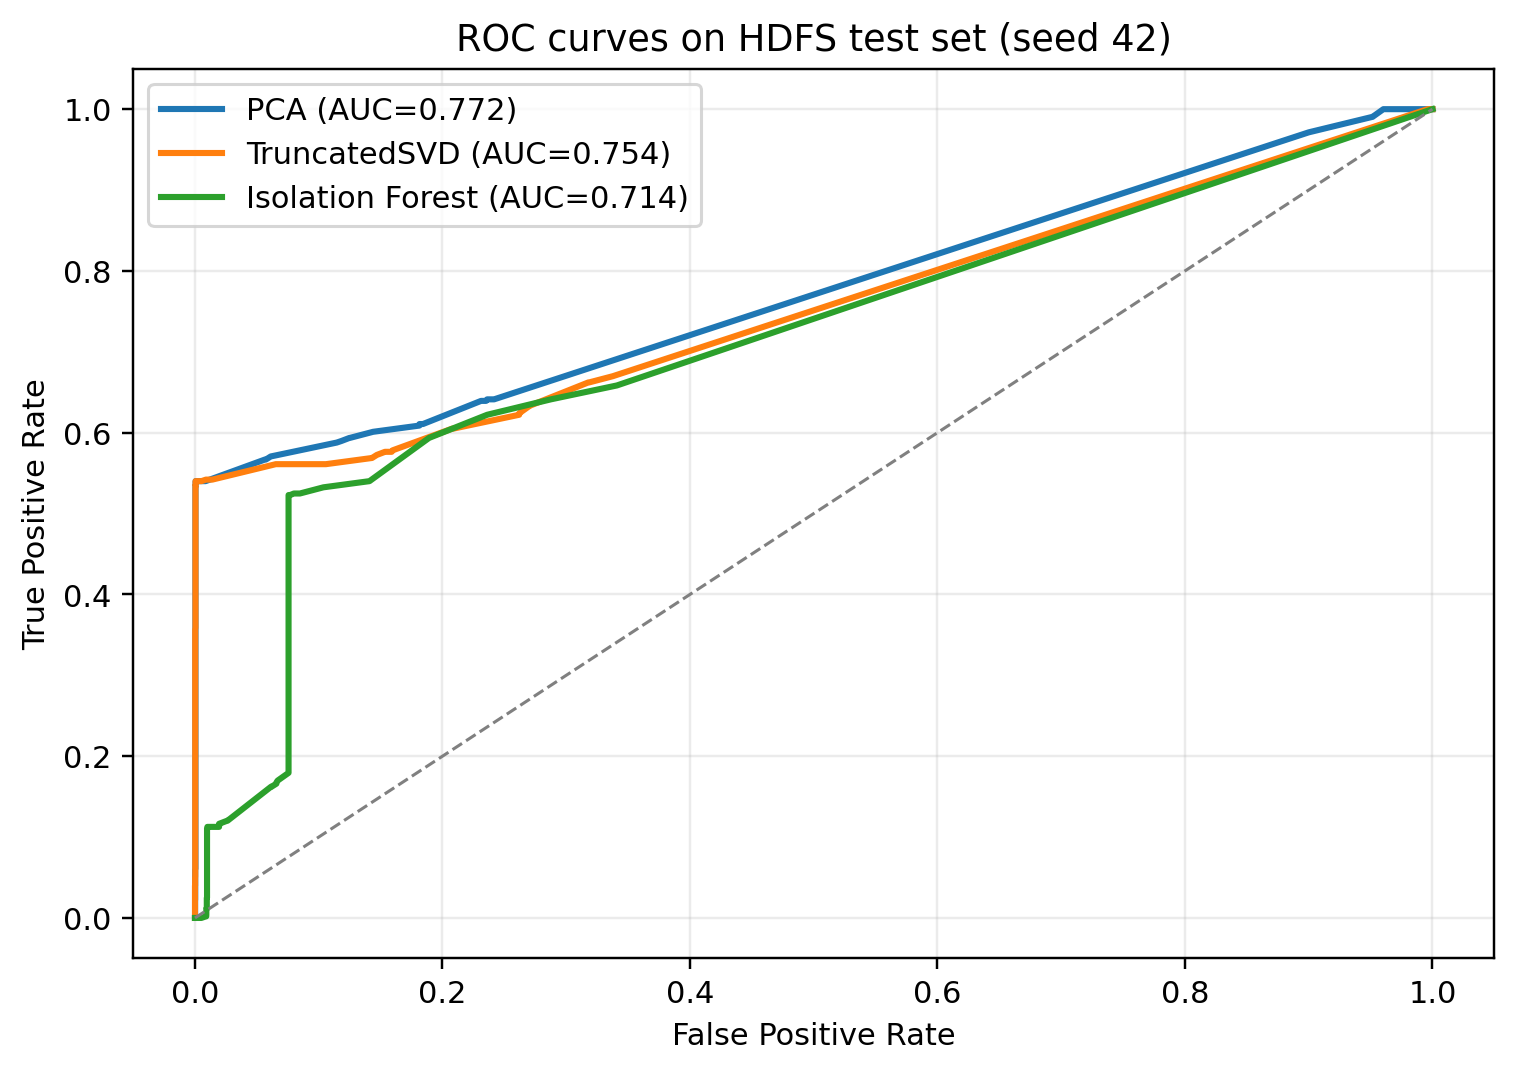
\includegraphics[width=\columnwidth]{roc_curves.png}
\caption{Đường ROC của các baseline trên tập kiểm thử HDFS}
\label{fig_roc}
\end{figure}

\begin{figure}[htbp]
\centering
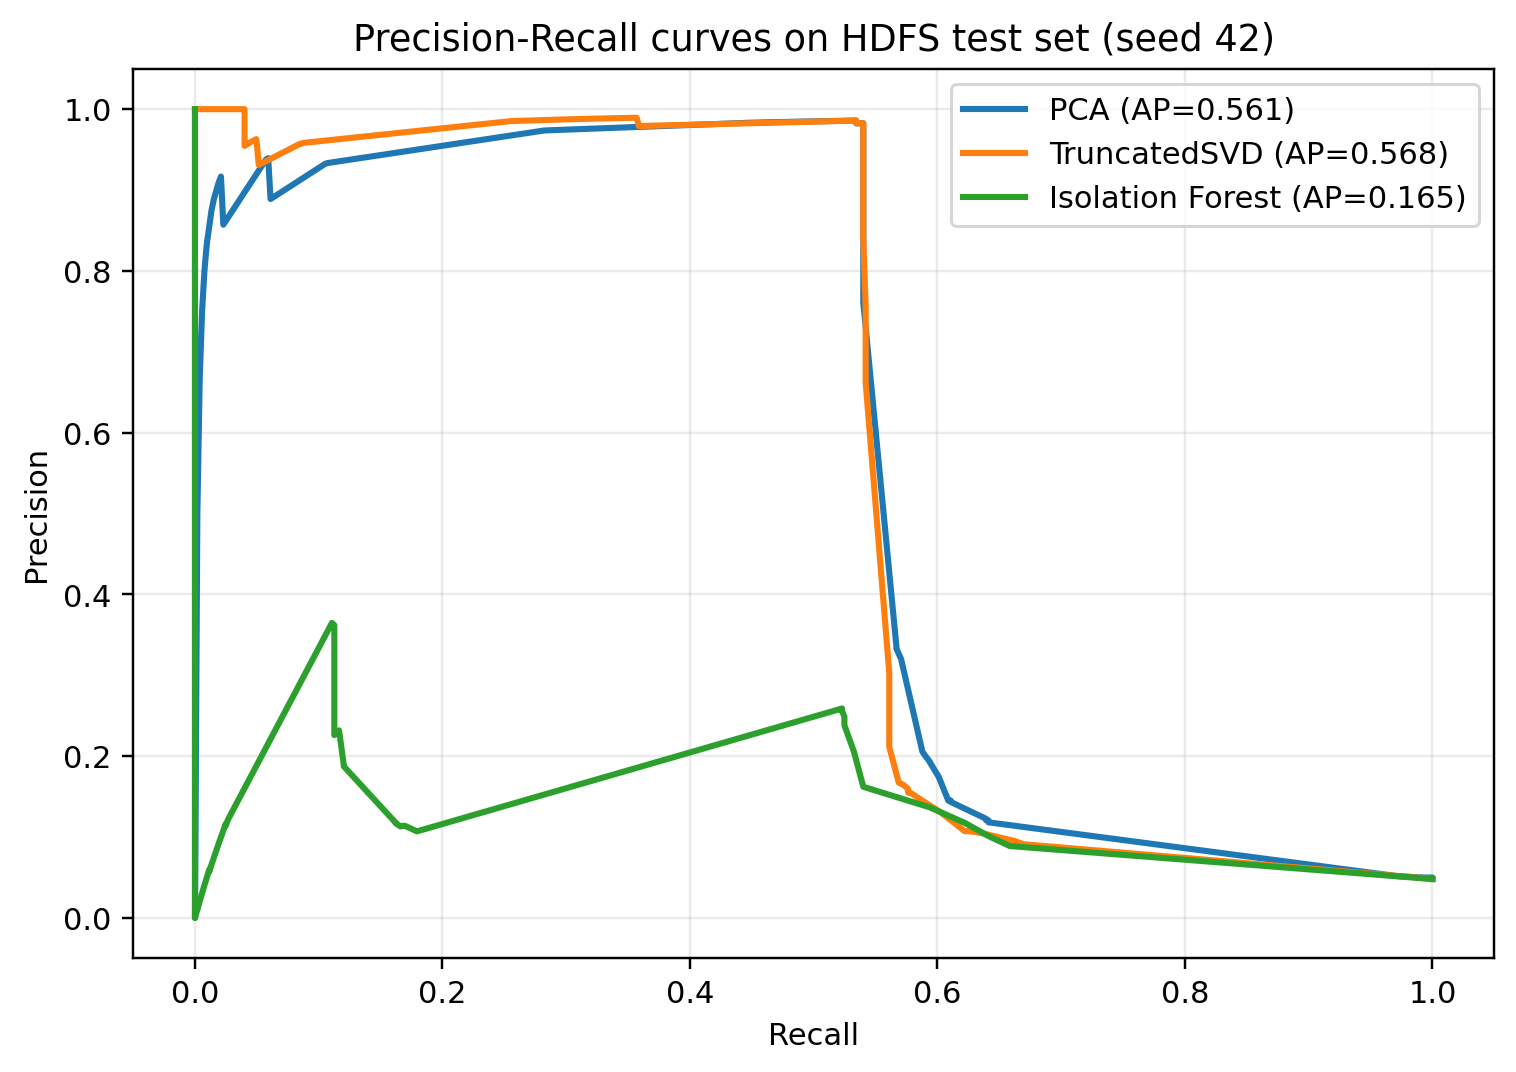
\includegraphics[width=\columnwidth]{pr_curves.png}
\caption{Đường Precision-Recall của các baseline trên tập kiểm thử HDFS}
\label{fig_pr}
\end{figure}

\begin{figure*}[!t]
\centering
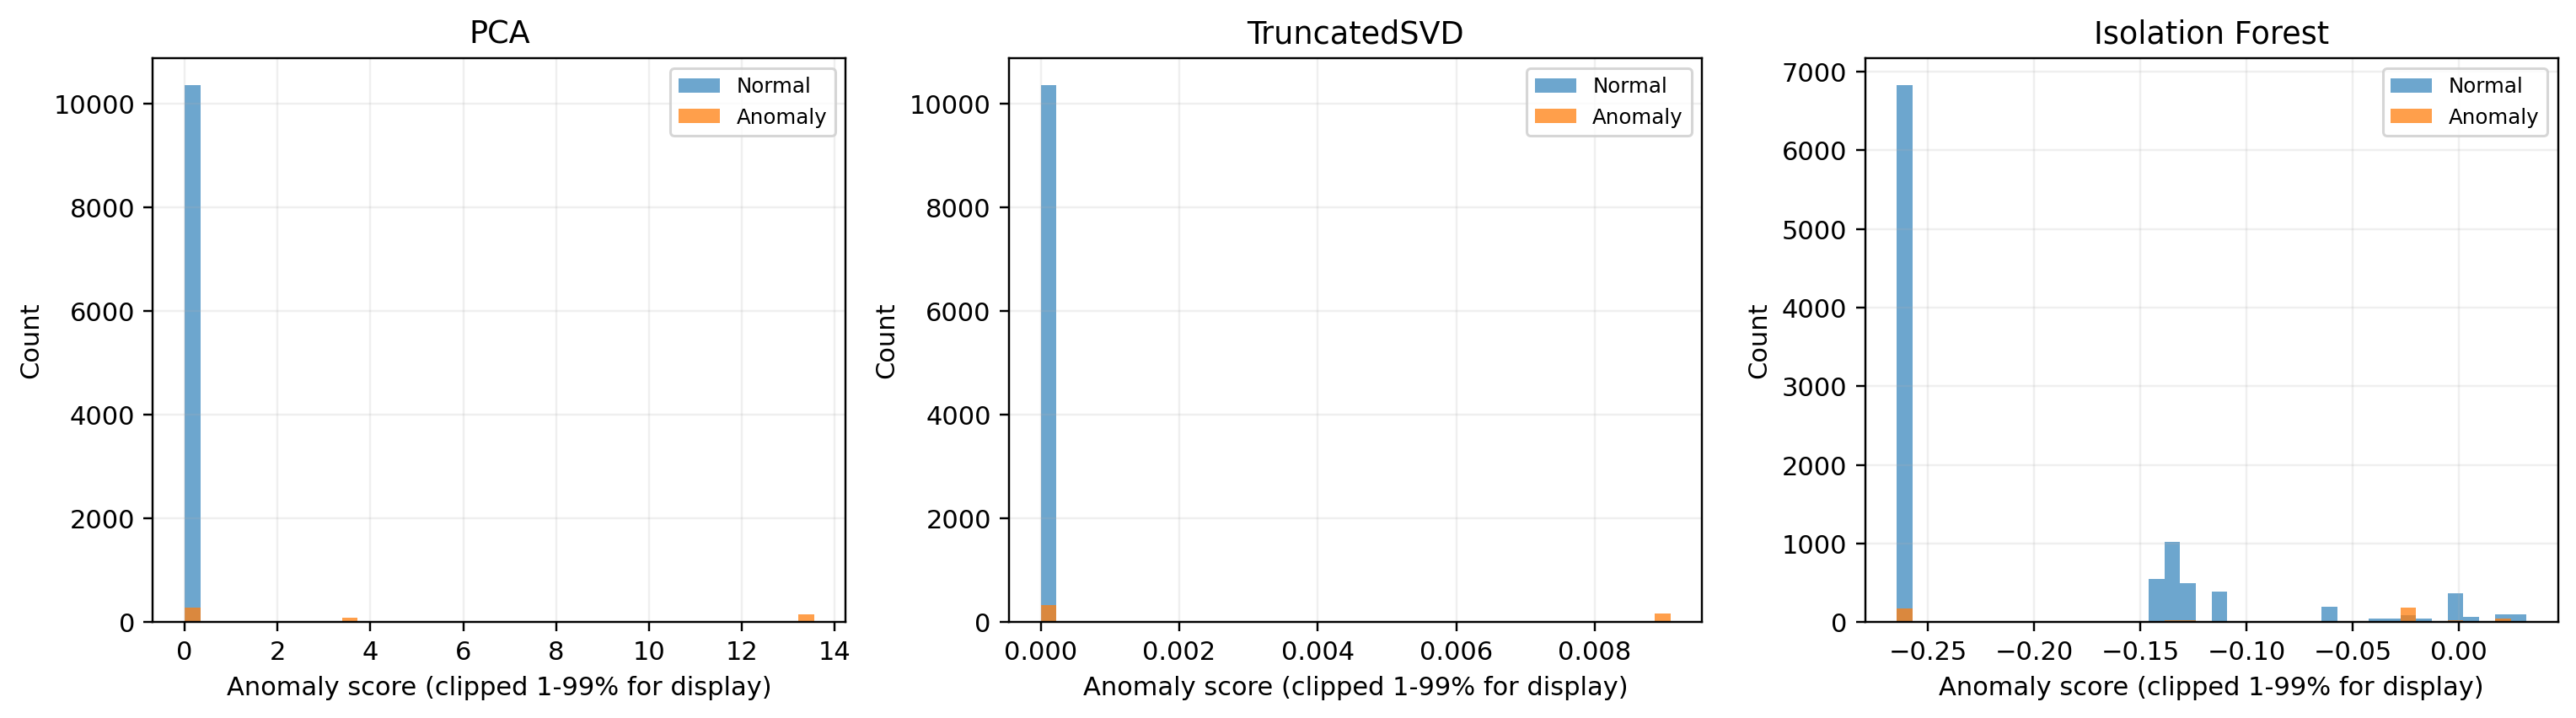
\includegraphics[width=0.95\textwidth]{score_distributions.png}
\caption{Phân phối điểm bất thường của các baseline trên tập kiểm thử HDFS}
\label{fig_score_dist}
\end{figure*}

\begin{table}[htbp]
\caption{ROC-AUC và Average Precision trên tập kiểm thử HDFS (một lần chạy với seed 42 để minh hoạ; xếp hạng giữa các phương pháp ổn định khi đổi seed)}
\begin{center}
\begin{tabular}{lcc}
\toprule
\textbf{Phương pháp} & \textbf{ROC-AUC} & \textbf{Avg. Precision} \\
\midrule
PCA & 0.7722 & 0.5613 \\
TruncatedSVD & 0.7536 & 0.5676 \\
Isolation Forest & 0.7136 & 0.1645 \\
\bottomrule
\end{tabular}
\label{tab_auc_ap}
\end{center}
\end{table}

Bảng \ref{tab_auc_ap} cho thấy PCA và TruncatedSVD có khả năng xếp hạng bất thường tốt hơn Isolation Forest, đặc biệt theo Average Precision. Điều này phù hợp với kết quả F1-score: các phương pháp reconstruction tận dụng tốt hơn cấu trúc event sau khi parse bằng Drain3, trong khi Isolation Forest gặp khó khăn với biểu diễn event rời rạc.

\begin{table}[htbp]
\caption{Độ nhạy F1-score theo percentile chọn ngưỡng (một lần chạy với seed 42 để minh hoạ chiều biến thiên; con số tuyệt đối có thể dịch chuyển theo seed như báo cáo ở Bảng \ref{tab_cross_dataset})}
\begin{center}
\begin{tabular}{lcccc}
\toprule
\textbf{Phương pháp} & \textbf{90} & \textbf{95} & \textbf{97} & \textbf{99} \\
\midrule
PCA & 0.4102 & 0.6317 & 0.6317 & 0.6317 \\
TruncatedSVD & 0.2498 & 0.3070 & 0.6297 & 0.6297 \\
Isolation Forest & 0.3278 & 0.1465 & 0.1465 & 0.0222 \\
\bottomrule
\end{tabular}
\label{tab_threshold_sensitivity}
\end{center}
\end{table}

Bảng \ref{tab_threshold_sensitivity} cho thấy hiệu năng phụ thuộc đáng kể vào cách chọn ngưỡng. Với PCA và TruncatedSVD, percentile cao hơn làm tăng Precision và cải thiện F1-score trong thiết lập này. Ngược lại, Isolation Forest nhạy hơn với ngưỡng và suy giảm mạnh ở percentile 99. Vì vậy, khi triển khai thực tế, ngưỡng cảnh báo cần được hiệu chỉnh bằng validation set hoặc theo chi phí vận hành giữa cảnh báo giả và bỏ sót sự cố.

\subsection{Đánh giá chéo trên BGL}
\label{sec:bgl}
Để kiểm tra mức độ khái quát của pipeline ngoài HDFS, chúng tôi đánh giá lại tất cả phương pháp trên BGL \cite{b18,b12}, một bộ log siêu máy tính có đặc trưng rất khác HDFS: vocabulary lớn hơn, không có Block ID nên phải dùng cửa sổ cố định, và tỷ lệ anomaly cao hơn nhiều. Cụ thể, từ 500.000 dòng đầu của BGL, Drain3 sinh 198 event template; chúng tôi gom thành cửa sổ không chồng lấn $W{=}100$ dòng, thu được 5.000 cửa sổ với 2.343 cửa sổ bất thường (47\%). Mọi phương pháp dùng cùng siêu tham số như khi chạy trên HDFS, chỉ thay grouping. Bảng \ref{tab_cross_dataset} đặt kết quả BGL cạnh kết quả HDFS để so sánh trực tiếp.

\begin{table*}[!t]
\caption{So sánh chéo các nhánh chấm điểm trên cùng pipeline Drain3 cho HDFS và BGL, trung bình $\pm$ độ lệch chuẩn trên 5 random seed (21, 42, 84, 123, 777). HDFS reconstruction baseline dùng 500k dòng/36.305 chuỗi BlockId; HDFS sequence model dùng 200k dòng/15.639 chuỗi; BGL dùng 500k dòng/5.000 cửa sổ $W{=}100$.}
\centering
\scriptsize
\setlength{\tabcolsep}{3pt}
\begin{tabular}{l ccc ccc}
\toprule
& \multicolumn{3}{c}{\textbf{HDFS}} & \multicolumn{3}{c}{\textbf{BGL}} \\
\cmidrule(lr){2-4} \cmidrule(lr){5-7}
\textbf{Phương pháp} & \textbf{Precision} & \textbf{Recall} & \textbf{F1} & \textbf{Precision} & \textbf{Recall} & \textbf{F1} \\
\midrule
PCA & $0.6274 \pm 0.1944$ & $0.5450 \pm 0.0055$ & $0.5711 \pm 0.0944$ & $0.9473 \pm 0.0113$ & $0.8976 \pm 0.0144$ & $0.9217 \pm 0.0098$ \\
TruncatedSVD & $0.4298 \pm 0.2555$ & $0.5527 \pm 0.0106$ & $0.4540 \pm 0.1366$ & $0.9462 \pm 0.0051$ & $0.9255 \pm 0.0228$ & $0.9356 \pm 0.0117$ \\
Isolation Forest & $0.1726 \pm 0.0146$ & $0.1080 \pm 0.0084$ & $0.1328 \pm 0.0103$ & $0.1110 \pm 0.0171$ & $0.0248 \pm 0.0045$ & $0.0404 \pm 0.0070$ \\
\midrule
Transformer (unsup.) & $0.2094 \pm 0.0490$ & $0.2982 \pm 0.0892$ & $0.2458 \pm 0.0639$ & $0.9422 \pm 0.0110$ & $0.9073 \pm 0.0216$ & $0.9242 \pm 0.0085$ \\
Transformer (val-tuned) & $0.5102 \pm 0.1497$ & $0.2365 \pm 0.1156$ & $0.2950 \pm 0.0693$ & $0.9841 \pm 0.0017$ & $0.8975 \pm 0.0157$ & $0.9388 \pm 0.0080$ \\
DeepLog (top-k) & $0.9817 \pm 0.0188$ & $0.3013 \pm 0.0167$ & $0.4608 \pm 0.0196$ & $0.9658 \pm 0.0068$ & $\mathbf{0.9991 \pm 0.0012}$ & $\mathbf{0.9822 \pm 0.0035}$ \\
DeepLog (NLL) & $0.2614 \pm 0.0127$ & $0.3629 \pm 0.0276$ & $0.3037 \pm 0.0165$ & $0.9393 \pm 0.0072$ & $0.9312 \pm 0.0236$ & $0.9351 \pm 0.0121$ \\
\bottomrule
\end{tabular}
\label{tab_cross_dataset}
\end{table*}

Bảng \ref{tab_cross_dataset} cho thấy ba điểm đảo chiều khi chuyển từ HDFS sang BGL. Thứ nhất, DeepLog top-k vọt từ F1 $0.4608$ lên $0.9822 \pm 0.0035$ với Recall gần như tuyệt đối ($0.9991 \pm 0.0012$): cấu hình LSTM mặc định ($g{=}10$, $K{=}9$) khi gặp vocabulary lớn hơn (198 vs 137 template) và cửa sổ dài hơn ($W{=}100$ vs $\sim$13.77 event) phát huy lợi thế next-event prediction rõ rệt. Thứ hai, Transformer val-tuned đạt F1 $0.9388 \pm 0.0080$, vượt nhẹ các baseline reconstruction. Thứ ba, Isolation Forest tiếp tục yếu trên cả hai dataset, khẳng định tín hiệu bất thường nằm trong cấu trúc chuỗi chứ không chỉ tần suất event. Tóm lại, cùng một pipeline Drain3 $\rightarrow$ chuỗi event $\rightarrow$ scoring vận hành ổn định trên hai bộ log rất khác nhau; việc chọn nhánh chấm điểm phụ thuộc trực tiếp vào đặc trưng dữ liệu.

\subsection{Ablation studies}
\label{sec:ablation}
Để hiểu vai trò của ba siêu tham số then chốt, chúng tôi tiến hành ba khảo sát ablation với seed 42 trên HDFS 200k: (i) ngưỡng tương đồng Drain3 $\theta$, (ii) hyperparameter $K$ của DeepLog top-k, (iii) tỷ lệ mask $r$ của Transformer. Bảng \ref{tab_ablation} tóm tắt kết quả.

\begin{table}[!t]
\caption{Ablation siêu tham số trên HDFS 200k (seed 42)}
\begin{center}
\scriptsize
\setlength{\tabcolsep}{3pt}
\begin{tabular}{lcccc}
\toprule
\textbf{Cấu hình} & \textbf{Templates} & \textbf{Precision} & \textbf{Recall} & \textbf{F1} \\
\midrule
\multicolumn{5}{l}{\textit{(A) Drain3 $\theta$, đo trên PCA reconstruction}} \\
$\theta=0.3$ & 25 & 0.3695 & 0.5215 & 0.4325 \\
$\theta=0.5$ \textbf{(default)} & 68 & 0.4070 & 0.5550 & \textbf{0.4696} \\
$\theta=0.7$ & 2455 & 0.1000 & 0.0287 & 0.0446 \\
\midrule
\multicolumn{5}{l}{\textit{(B) DeepLog top-k}} \\
$K=1$ & 68 & 0.0466 & 0.6403 & 0.0869 \\
$K=3$ & 68 & 0.9091 & 0.2878 & 0.4372 \\
$K=5$ & 68 & 0.9524 & 0.2878 & 0.4420 \\
$K=9$ \textbf{(default)} & 68 & 0.9756 & 0.2878 & \textbf{0.4444} \\
$K=15$ & 68 & 0.9750 & 0.2806 & 0.4358 \\
\midrule
\multicolumn{5}{l}{\textit{(C) Transformer mask ratio $r$}} \\
$r=0.10$ & 68 & 0.1615 & 0.2230 & 0.1873 \\
$r=0.15$ \textbf{(default)} & 68 & 0.1968 & 0.2662 & \textbf{0.2263} \\
$r=0.20$ & 68 & 0.1711 & 0.2302 & 0.1963 \\
$r=0.30$ & 68 & 0.1701 & 0.2374 & 0.1982 \\
\bottomrule
\end{tabular}
\label{tab_ablation}
\end{center}
\end{table}

Kết quả ablation cung cấp ba góc nhìn cụ thể. (A) Ngưỡng Drain3 ảnh hưởng mạnh tới chất lượng pipeline: $\theta{=}0.3$ over-merge (chỉ 25 template, F1 thấp do trộn nhiều sự kiện khác nhau); $\theta{=}0.7$ gây template explosion (2.455 template, F1 sụp đổ về $0.0446$); $\theta{=}0.5$ là sweet spot, cũng là giá trị mặc định được dùng xuyên suốt bài báo. (B) DeepLog top-k bão hòa quanh $K{=}5$--$9$ với precision cao và recall ổn định; $K{=}1$ quá khắt khe (precision 0.05), $K{=}15$ bắt đầu nhỡ anomaly. (C) Mask ratio cho Transformer mini đạt F1 cao nhất ở giá trị mặc định $r{=}0.15$ — trùng với mask ratio kinh điển của BERT \cite{b4}; tăng $r$ lên 0.20--0.30 giảm hiệu quả vì quá nhiều token bị che. Hình \ref{fig_vocab_growth} bổ sung phân tích vocabulary growth: số template tăng từ 13 (5k dòng) lên 137 (500k dòng) theo dạng tăng nhanh dần, cho thấy benchmark HDFS thực sự sinh thêm template khi tăng quy mô dữ liệu.

\begin{figure}[!t]
\centering
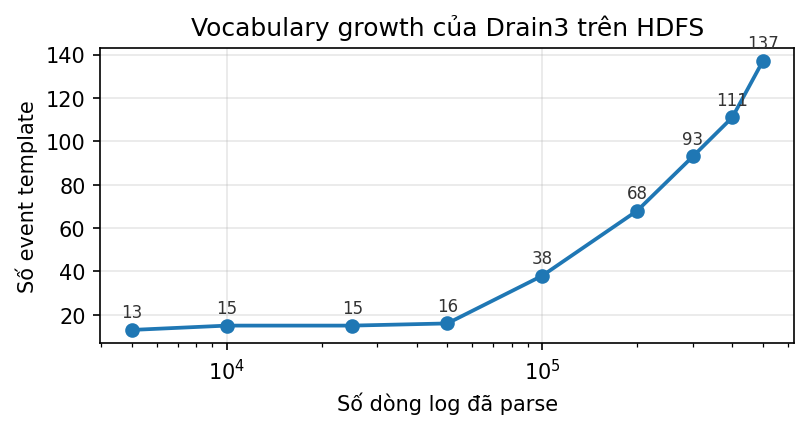
\includegraphics[width=0.9\columnwidth]{vocab_growth.png}
\caption{Số event template Drain3 sinh ra theo số dòng log HDFS đã parse (Drain3 $\theta{=}0.5$, depth 4)}
\label{fig_vocab_growth}
\end{figure}

\subsection{Phân tích lỗi dự kiến}
Do benchmark HDFS không cung cấp mô tả chi tiết từng loại lỗi ở cấp nghiệp vụ như LMS, bài báo phân tích lỗi ở mức pattern dự kiến dựa trên điểm bất thường và đặc tính của pipeline. Bảng \ref{tab_error_analysis} tóm tắt các dạng lỗi có khả năng xuất hiện khi chuyển pipeline sang môi trường vận hành thực tế.

\begin{table}[!t]
\caption{Phân tích lỗi dự kiến của pipeline}
\begin{center}
\scriptsize
\begin{tabular}{p{1.65cm}p{2.45cm}p{2.35cm}}
\toprule
\textbf{Dạng lỗi} & \textbf{Nguyên nhân có thể} & \textbf{Hướng giảm thiểu} \\
\midrule
False positive với chuỗi hiếm & Chuỗi bình thường nhưng ít xuất hiện trong train, ví dụ hoạt động quản trị hoặc kỳ thi & Tách profile theo vai trò người dùng, thời điểm và dịch vụ \\
False positive với chuỗi dài & Reconstruction error bị ảnh hưởng bởi số lượng event hoặc burst traffic & Chuẩn hóa theo độ dài chuỗi, dùng cửa sổ nghiệp vụ ổn định \\
False negative & Anomaly dùng các event template phổ biến nên không lệch nhiều về tần suất & Bổ sung mô hình chuỗi như DeepLog/LogBERT và đặc trưng thời gian \\
Template collision & Drain3 gộp hai loại log khác nghĩa vào cùng template & Tinh chỉnh ngưỡng Drain3, kiểm tra template entropy và template hiếm \\
Domain shift LMS & HDFS không chứa hành vi nghiệp vụ như đăng nhập, nộp bài, làm quiz & Thu thập log LMS đã ẩn danh và đánh giá theo session/user/window \\
\bottomrule
\end{tabular}
\label{tab_error_analysis}
\end{center}
\end{table}

\subsection{Chi phí triển khai và độ trễ suy luận}
Một hệ thống giám sát log thực tế cần đo độ trễ cảnh báo bên cạnh F1-score. Để có chuẩn so sánh, chúng tôi đo per-sample inference latency cho từng nhánh với batch size 1 trên RTX 4050 Laptop (Drain3 và baseline thuần CPU; DeepLog/Transformer đo cả CPU và GPU), warm-up 50 lần và lấy trung bình trên 1.000 mẫu HDFS (Bảng \ref{tab_latency}).

\begin{table}[!t]
\caption{Per-sample inference latency, batch 1, trung bình trên 1.000 mẫu HDFS (đơn vị: ms)}
\begin{center}
\scriptsize
\setlength{\tabcolsep}{3pt}
\begin{tabular}{lcccc}
\toprule
\textbf{Nhánh} & \textbf{Mean} & \textbf{p95} & \textbf{p99} & \textbf{Throughput} \\
\midrule
Drain3 parse 1 dòng & 0.004 & 0.011 & 0.035 & 227.988 logs/s \\
PCA reconstruction & 0.055 & 0.082 & 0.173 & 18.079 chuỗi/s \\
TruncatedSVD & 0.145 & 0.280 & 0.397 & 6.883 chuỗi/s \\
Isolation Forest & 6.208 & 10.604 & 12.688 & 161 chuỗi/s \\
DeepLog (CPU) & 2.029 & 2.449 & 2.633 & 493 chuỗi/s \\
DeepLog (GPU) & 0.489 & 0.798 & 0.962 & 2.046 chuỗi/s \\
Transformer (CPU) & 2.711 & 3.247 & 3.733 & 369 chuỗi/s \\
Transformer (GPU) & 2.916 & 4.323 & 4.889 & 343 chuỗi/s \\
\bottomrule
\end{tabular}
\label{tab_latency}
\end{center}
\end{table}

Ba quan sát từ Bảng \ref{tab_latency}. Thứ nhất, Drain3 ở chế độ streaming xử lý $\sim$228k log/giây trên một core, không phải bottleneck của pipeline. Thứ hai, PCA và TruncatedSVD là nhánh nhanh nhất cho chấm điểm (<0.2ms/mẫu); Isolation Forest chậm hơn 100 lần do duyệt ensemble 200 cây và xử lý sparse vector. Thứ ba, DeepLog hưởng lợi rõ từ GPU (giảm từ 2.0ms xuống 0.49ms), trong khi Transformer cỡ nhỏ ở batch 1 không hưởng lợi nhiều vì overhead launch kernel $\sim$lớn hơn compute; với batch lớn (chế độ bulk scoring) GPU sẽ tăng tốc đáng kể. Bên cạnh độ trễ, tham số có ảnh hưởng lớn tới chất lượng gồm ngưỡng Drain3 $\theta$ (đã ablation ở §\ref{sec:ablation}), độ dài chuỗi/cửa sổ, mask ratio và ngưỡng percentile. Trong môi trường LMS, độ dài cửa sổ nên được chọn theo hành vi nghiệp vụ (phiên đăng nhập, truy cập tài liệu, nộp bài, làm bài, quản trị) thay vì cố định theo thời gian, để cảnh báo dễ truy nguyên hơn cho quản trị viên.

\begin{table}[htbp]
\caption{So sánh trade-off triển khai giữa các phương pháp}
\begin{center}
\scriptsize
\begin{tabular}{p{1.5cm}p{1.6cm}p{1.6cm}p{1.5cm}}
\toprule
\textbf{Phương pháp} & \textbf{Chi phí tính toán} & \textbf{Bộ nhớ} & \textbf{Nhận biết thứ tự} \\
\midrule
PCA & Thấp sau vector hóa & Trung bình do dense matrix & Không \\
TruncatedSVD & Thấp-trung bình, hợp sparse matrix & Thấp hơn PCA với dữ liệu thưa & Không \\
Isolation Forest & Thấp-trung bình & Trung bình & Không \\
Transformer & Cao hơn do attention và huấn luyện nhiều epoch & Cao hơn, phụ thuộc độ dài chuỗi & Có \\
\bottomrule
\end{tabular}
\label{tab_complexity_tradeoff}
\end{center}
\end{table}

Bảng \ref{tab_complexity_tradeoff} cho thấy các baseline nhẹ phù hợp cho bước kiểm chứng nhanh và triển khai tài nguyên hạn chế, nhưng không học được thứ tự event. Ngược lại, Transformer có khả năng học phụ thuộc chuỗi nhưng cần nhiều tài nguyên hơn và đòi hỏi thiết kế scoring cẩn thận. Đây là lý do bài báo đặt Transformer như hướng mở rộng thay vì kết luận rằng mô hình này đã vượt baseline trong thiết lập hiện tại.

\begin{table}[!t]
\caption{Thời gian chạy tham khảo trong notebook thực nghiệm}
\begin{center}
\scriptsize
\begin{tabular}{lcc}
\toprule
\textbf{Thành phần} & \textbf{Quy mô} & \textbf{Thời gian} \\
\midrule
Drain3 parsing & 500.000 dòng HDFS & 3.49 s \\
PCA baseline & 36.305 block & 0.74 s \\
TruncatedSVD baseline & 36.305 block & 1.29 s \\
Isolation Forest & 36.305 block & 1.16 s \\
Transformer training & 200.000 dòng HDFS & 10.75 s \\
\bottomrule
\end{tabular}
\label{tab_runtime}
\end{center}
\end{table}

Bảng \ref{tab_runtime} cho thấy pipeline baseline có thể chạy nhanh trên dữ liệu mẫu, trong khi Transformer cần thêm tài nguyên huấn luyện. Các con số này chỉ là thời gian tham khảo từ notebook và phụ thuộc phần cứng, nhưng đủ để cho thấy trade-off giữa baseline nhanh và mô hình chuỗi phức tạp.

\subsection{Phân tích ứng dụng trong giáo dục số}
Trong môi trường LMS, bất thường không chỉ là lỗi hệ thống mà còn có thể là dấu hiệu tấn công. Pipeline đề xuất có thể hỗ trợ các kịch bản sau:
\begin{itemize}
    \item \textbf{Tấn công dò mật khẩu:} Một chuỗi đăng nhập thất bại lặp lại từ nhiều IP hoặc nhiều tài khoản có thể tạo ra pattern khác biệt so với hành vi học tập bình thường.
    \item \textbf{Khai thác API:} Các request chứa tham số lạ, truy cập endpoint hiếm gặp hoặc template mới sinh ra từ Drain3 có thể được xem là tín hiệu cần kiểm tra.
    \item \textbf{Quá tải dịch vụ:} Chuỗi lỗi database timeout, HTTP 5xx và độ trễ tăng cao có thể phản ánh tình trạng quá tải vào thời điểm thi trực tuyến hoặc nộp bài tập.
    \item \textbf{Bất thường phiên người dùng:} Một tài khoản sinh viên đăng nhập từ nhiều vị trí, đổi thiết bị liên tục hoặc truy cập tài nguyên với nhịp độ bất thường có thể được đưa vào phân tích chuỗi.
\end{itemize}

Các kịch bản trên là phân tích ứng dụng, không thay thế cho thực nghiệm trên dữ liệu LMS thật. Khi triển khai thực tế, hệ thống cần kết hợp thêm cơ chế ẩn danh dữ liệu, kiểm soát quyền truy cập log và quy trình xác minh cảnh báo bởi quản trị viên.

\subsection{Threats to Validity}
Nghiên cứu hiện có một số nguy cơ ảnh hưởng tới độ tin cậy và khả năng khái quát hóa của kết quả. Thứ nhất, thực nghiệm chính được tái lập trên HDFS và BGL theo cùng pipeline (Bảng \ref{tab_cross_dataset}); log LMS thực tế vẫn là hướng mở rộng để kiểm tra khả năng tổng quát hóa liên miền. Thứ hai, dữ liệu HDFS không phản ánh đầy đủ đặc thù nghiệp vụ của LMS như lịch thi, nộp bài, truy cập học liệu hoặc hành vi người dùng đã ẩn danh, dẫn tới nguy cơ domain shift khi chuyển sang môi trường giáo dục số. Thứ ba, nhãn bất thường trong benchmark phụ thuộc vào cách gán nhãn theo Block ID; nếu nhãn nhiễu hoặc không bao quát mọi lỗi, metric có thể không phản ánh đầy đủ hiệu quả thực tế. Thứ tư, Drain3 có nguy cơ template collapse khi gộp nhiều mẫu log khác nhau vào cùng một template hoặc sinh quá nhiều template hiếm nếu ngưỡng không phù hợp. Thứ năm, kết quả phụ thuộc vào cách gom chuỗi và ngưỡng bất thường; phân tích độ nhạy cho thấy F1-score có thể thay đổi đáng kể theo percentile chọn ngưỡng. Thứ sáu, thử nghiệm Transformer hiện mới là mô hình masked event modeling nhỏ, chưa phải tái lập đầy đủ LogBERT gốc và chưa được tối ưu sâu về hyperparameter, scoring hoặc kích thước dữ liệu. Thứ bảy, baseline DeepLog đã được tái lập theo top-k và NLL threshold (cột HDFS và BGL của Bảng \ref{tab_cross_dataset}) nhưng vẫn dùng cấu hình LSTM mặc định ($g{=}10$, $K{=}9$); việc quét rộng hyperparameter của DeepLog cũng như tái lập đầy đủ LogAnomaly, LogRobust và PLELog vẫn được để dành cho mở rộng tiếp theo. Cuối cùng, bài báo chưa đánh giá độ trễ suy luận trong môi trường vận hành thời gian thực. Các yếu tố này được ghi nhận như định hướng cải thiện trong các phiên bản tiếp theo.

\subsection{Hạn chế triển khai}
Khi triển khai trong hạ tầng giáo dục số, hệ thống cần xử lý thêm các ràng buộc về riêng tư dữ liệu, phân quyền truy cập log và quy trình xác minh cảnh báo bởi quản trị viên. Log LMS có thể chứa user ID, email, IP, session ID hoặc hành vi học tập, vì vậy cần ẩn danh trước khi huấn luyện. Ngoài ra, mô hình hiện chưa tự động giải thích nguyên nhân theo ngôn ngữ dễ hiểu cho quản trị viên; phần giải thích cảnh báo nên được xem là hướng mở rộng sau khi pipeline phát hiện đã được kiểm chứng trên dữ liệu thực.

\section{Kết luận}
Bài báo đã trình bày một pipeline phát hiện bất thường log dựa trên Drain3 và phân tích chuỗi sự kiện, đánh giá song song bốn nhánh chấm điểm (PCA/SVD reconstruction, Isolation Forest, DeepLog next-event prediction, Transformer masked event modeling) trên HDFS và BGL với cùng giao thức 5 random seed. Trên HDFS, PCA dẫn đầu nhờ chuỗi ngắn và vocabulary nhỏ; trên BGL, DeepLog top-k đạt F1 $\sim$0.98 và Transformer val-tuned vượt nhẹ PCA, cho thấy kết quả khiêm tốn của mô hình chuỗi trên HDFS chủ yếu phản ánh đặc trưng compact của benchmark hơn là khuyết tật của hướng tiếp cận. Đối với giáo dục số, kết quả hiện là bước kiểm chứng pipeline ở cấp hạ tầng, chưa phải bằng chứng triển khai trên LMS thật. Ba hướng phát triển tiếp theo gồm: (i) thu thập và đánh giá trên log LMS thực tế đã ẩn danh (Moodle, Keycloak, Nginx, API gateway) với session grouping theo người dùng; (ii) thay event template ID bằng semantic embedding (SentenceTransformer trên nội dung template) để pipeline robust hơn với log biến động; (iii) bổ sung cơ chế giải thích cảnh báo (attention heatmap, anomalous subsequence, root-cause candidate ranking) phù hợp với nhu cầu vận hành của quản trị viên giáo dục số. Song song, cần tái lập đầy đủ LogBERT với hypersphere objective và quét rộng hyperparameter DeepLog.

\begin{thebibliography}{00}
\bibitem{b1} M. Du, F. Li, G. Zheng, and V. Srikumar, ``DeepLog: Anomaly Detection and Diagnosis from System Logs through Deep Learning,'' in \textit{Proc. ACM CCS}, 2017.
\bibitem{b2} H. Guo, S. Yuan, and X. Wu, ``LogBERT: Log Anomaly Detection via BERT,'' in \textit{Proc. International Joint Conference on Neural Networks (IJCNN)}, 2021.
\bibitem{b3} P. He, J. Zhu, Z. Zheng, and M. R. Lyu, ``Drain: An Online Log Parsing Approach with Fixed Depth Tree,'' in \textit{Proc. IEEE International Conference on Web Services (ICWS)}, 2017.
\bibitem{b4} A. Vaswani et al., ``Attention Is All You Need,'' in \textit{Proc. NeurIPS}, 2017.
\bibitem{b5} S. He, J. Zhu, P. He, and M. R. Lyu, ``Experience Report: System Log Analysis for Anomaly Detection,'' in \textit{Proc. IEEE International Symposium on Software Reliability Engineering (ISSRE)}, 2016.
\bibitem{b6} J. Zhu et al., ``Tools and Benchmarks for Automated Log Parsing,'' in \textit{Proc. IEEE/ACM International Conference on Software Engineering (ICSE)}, 2019.
\bibitem{b7} V. H. Le and H. Zhang, ``Log Parsing with Prompt-based Few-shot Learning,'' in \textit{Proc. IEEE/ACM International Conference on Software Engineering (ICSE)}, 2023.
\bibitem{b8} T. Zhang, X. Huang, W. Zhao, S. Bian, and P. Du, ``LogPrompt: A Log-based Anomaly Detection Framework Using Prompts,'' in \textit{Proc. International Joint Conference on Neural Networks (IJCNN)}, 2023.
\bibitem{b9} X. Han, S. Yuan, and M. Trabelsi, ``LogGPT: Log Anomaly Detection via GPT,'' in \textit{Proc. IEEE International Conference on Big Data}, 2023.
\bibitem{b10} V. Chandola, A. Banerjee, and V. Kumar, ``Anomaly Detection: A Survey,'' \textit{ACM Computing Surveys}, vol. 41, no. 3, pp. 1--58, 2009.
\bibitem{b11} F. T. Liu, K. M. Ting, and Z.-H. Zhou, ``Isolation Forest,'' in \textit{Proc. IEEE International Conference on Data Mining (ICDM)}, 2008.
\bibitem{b12} J. Zhu, S. He, J. Liu, M. R. Lyu, and P. He, ``Loghub: A Large Collection of System Log Datasets for AI-driven Log Analytics,'' in \textit{Proc. IEEE International Symposium on Software Reliability Engineering (ISSRE)}, pp. 355--366, 2023.
\bibitem{b13} W. Meng et al., ``LogAnomaly: Unsupervised Detection of Sequential and Quantitative Anomalies in Unstructured Logs,'' in \textit{Proc. International Joint Conference on Artificial Intelligence (IJCAI)}, pp. 4739--4745, 2019.
\bibitem{b14} X. Zhang et al., ``Robust Log-Based Anomaly Detection on Unstable Log Data,'' in \textit{Proc. ACM Joint Meeting on European Software Engineering Conference and Symposium on the Foundations of Software Engineering (ESEC/FSE)}, 2019.
\bibitem{b15} L. Yang et al., ``Semi-Supervised Log-Based Anomaly Detection via Probabilistic Label Estimation,'' in \textit{Proc. IEEE/ACM International Conference on Software Engineering (ICSE)}, 2021.
\bibitem{b16} M. Landauer, S. Onder, F. Skopik, and M. Wurzenberger, ``Deep Learning for Anomaly Detection in Log Data: A Survey,'' \textit{Machine Learning with Applications}, vol. 12, 2023.
\bibitem{b17} I. Loshchilov and F. Hutter, ``Decoupled Weight Decay Regularization,'' in \textit{Proc. International Conference on Learning Representations (ICLR)}, 2019.
\bibitem{b18} A. Oliner and J. Stearley, ``What Supercomputers Say: A Study of Five System Logs,'' in \textit{Proc. IEEE/IFIP International Conference on Dependable Systems and Networks (DSN)}, 2007.
\end{thebibliography}

\end{document}
